\documentclass[12pt]{article}
\usepackage[margin=1in]{geometry}
\usepackage{amsmath}
\usepackage{booktabs}
\usepackage{graphicx}
\usepackage{tikz}
\usepackage{mathtools}  
\usepackage{xfrac}  
\usepackage[section]{placeins}
\usetikzlibrary{automata,positioning,arrows}
\newcommand\tab[1][1cm]{\hspace*{#1}}
\newcommand\n{\newline}
\newcommand\partiald[2]{
    \frac{\partial #1}{\partial #2}
}
\newcommand\ra{\rightarrow}

\begin{document}
CS7347 Test 2, Noah Gardner, 000843905\n

% P1
\section*{Question 1}
\textbf{[Points 15]} A grammar is ambiguous if it can generate a
string two or more ways. In other words, a string generated by the
grammar does not have a unique parse tree.

Given grammar:

\begin{tabular}{lll}
      S & $\rightarrow$ & a B $|$ b A         \\
      A & $\rightarrow$ & a $|$ a S $|$ b A A \\
      B & $\rightarrow$ & b $|$ b S $|$ a B B \\
\end{tabular}

Is the above grammar ambiguous? Provide an example and show parse tree
to validate your answer.

% P2
\newpage
\section*{Question 2}
\textbf{[Points 15]} Describe issue of BLEU Score. Given candidate
translation sentences and their references below, compute modified BLEU
score.

\textbf{Candidate 1:} It is a guide to action which ensures that the
military always obeys the commands of the party.

\textbf{Candidate 2:} It is to ensure the troops forever hearing the
activity guidebook that party direct.

\textbf{Reference 1:} It is a guide to action that ensures that the
military will forever heed Party commands.

\textbf{Reference 2:} It is the guiding principle which guarantees
the military forces always being under the command of the Party.

\textbf{Reference 3:} It is the practical guide for the army always to
heed the directions of the party.

Evaluate your translation model performance using BLEU score where
$n$-gram order, $N=2$. Please show the best reference during your
computation.

% P3
\newpage
\section*{Question 3}
\textbf{[Points 10]} Given a grammar below

\begin{tabular}{lll}
      \hline
      NP  & $\rightarrow$ & Det $|$ Nom                            \\
      Nom & $\rightarrow$ & AP $|$ Nom                             \\
      AP  & $\rightarrow$ & Adv $|$ A                              \\
      \hline
      Det & $\rightarrow$ & a $|$ an                               \\
      Adv & $\rightarrow$ & very $|$ extremely                     \\
      AP  & $\rightarrow$ & heavy $|$ orange $|$ tall              \\
      A   & $\rightarrow$ & heavy $|$ orange $|$ tall $|$ muscular \\
      Nom & $\rightarrow$ & book $|$ orange $|$ man                \\
      \hline
\end{tabular}

Show a parse tree for the following sentences:

\textbf{Sentence 1:} A very heavy orange book

\textbf{Sentence 2:} A very tall extremely muscular man

\textbf{Answer:}

\begin{figure}[!ht]
      \centering
      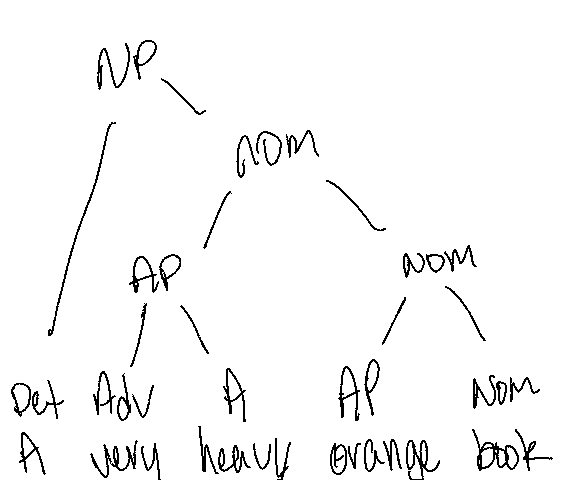
\includegraphics[width=0.5\textwidth]{assets/test2/p3a.png}
\end{figure}

\begin{figure}[!ht]
      \centering
      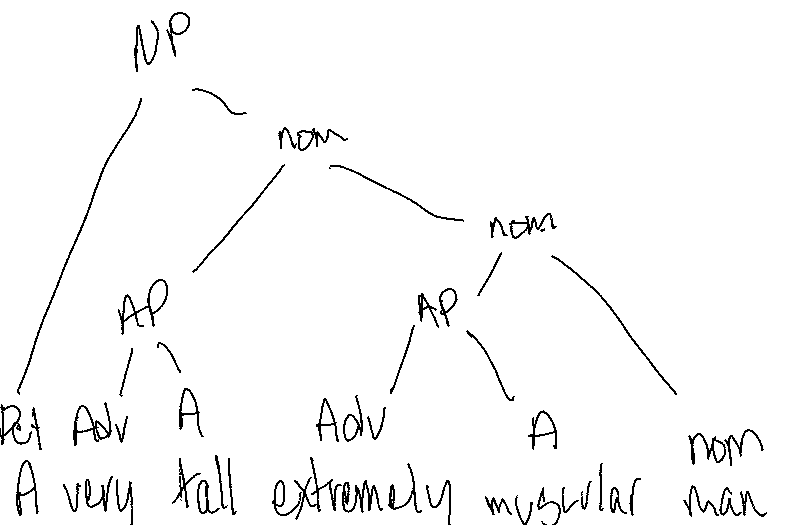
\includegraphics[width=0.5\textwidth]{assets/test2/p3b.png}
\end{figure}

% P4
\newpage
\section*{Question 4}
\textbf{[Points 5]} Write down the differences between attachment
ambiguity and coordination ambiguity.

% P5
\newpage
\section*{Question 5}
\textbf{[Points 15]} Suppose you build two summarizer systems, and
your systems generates the following summary. You named your summarizer as
S1 and S2, respectively. You are also given reference summary below.

\textbf{S1 Summary:} neymar scored his side's second goal with a
curling free kick, and 15 minutes to play in the 2-2 draw at sevilla
on saturday night, according to reports in spain.

\textbf{S2 Summary:} barcelona's neymar substituted in 2-2 draw at
sevilla on saturday night, spain's kamui kobayashi claims a late free
kick in the champions league after his second goal with the score

\textbf{Reference summary:} neymar was taken off with barcelona 2-1 up against sevilla. the brazil
captain was visibly angry, and barca went on to draw 2-2. neymar has been replaced 15 times in
34 games this season. click here for all the latest barcelona news.

Please compute the performance of your system using ROUGE-1 and ROUGE-2 - precision,
recall, and f1 score metrics and compare both systems with respective ROUGE metrics (e.g.,
ROUGE-1 S1 vs. ROUGE-1 S2). Based on your comparison, which one of the ROUGE metrics
would you select to evaluate your system performance?

% P6
\newpage
\section*{Question 6}
\textbf{[Points 5]} Given a grammar below

\begin{tabular}{|lll|}
      \hline
      S  & $\rightarrow$ & NP VP \\
      \hline
      VP & $\rightarrow$ & Vi    \\
      VP & $\rightarrow$ & Vt NP \\
      VP & $\rightarrow$ & VP PP \\
      \hline
      NP & $\rightarrow$ & DT NN \\
      NP & $\rightarrow$ & NP PP \\
      \hline
      PP & $\rightarrow$ & IN NP \\
      \hline
\end{tabular}

\begin{tabular}{|lll|}
      \hline
      Vi & $\rightarrow$ & 'sleeps'    \\
      Vt & $\rightarrow$ & 'saw'       \\
      \hline
      NN & $\rightarrow$ & 'man'       \\
      NN & $\rightarrow$ & 'woman'     \\
      NN & $\rightarrow$ & 'telescope' \\
      NN & $\rightarrow$ & 'dog'       \\
      \hline
      DT & $\rightarrow$ & 'the'       \\
      \hline
      IN & $\rightarrow$ & 'with'      \\
      IN & $\rightarrow$ & 'in'        \\
      \hline
\end{tabular}

Show that this grammar is ambiguous and produces two different parse
tree for the following sentence.

\textbf{Sentence:} the man saw the dog with the telescope

\textbf{Answer:}

\begin{figure}[!ht]
      \centering
      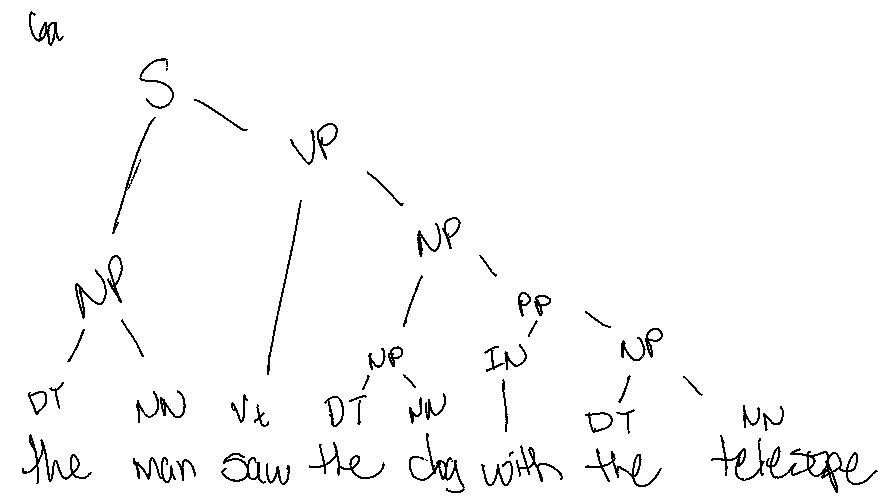
\includegraphics[width=0.5\textwidth]{assets/test2/p6a.png}
\end{figure}

\begin{figure}[!ht]
      \centering
      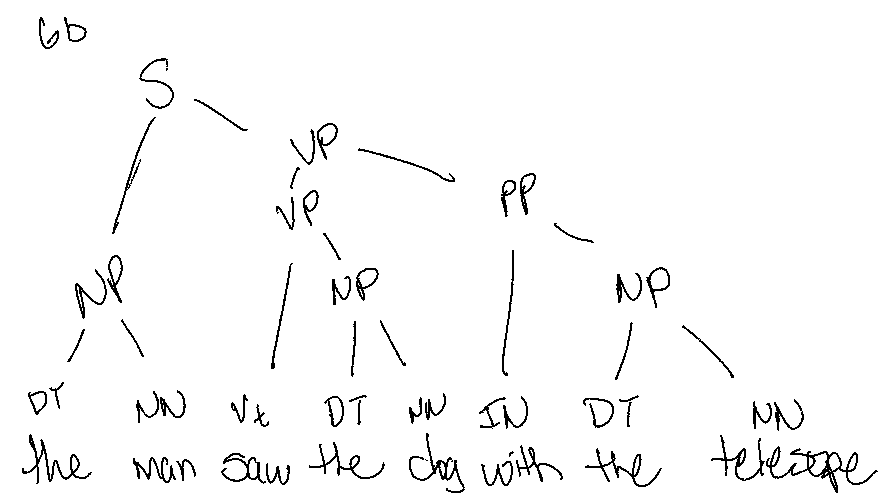
\includegraphics[width=0.5\textwidth]{assets/test2/p6b.png}
\end{figure}

% P7
\newpage
\section*{Question 7}
\textbf{[Points 20]} Evaluate the following example and compute precision,
recall and F1 scores.

\begin{figure}[!ht]
      \centering
      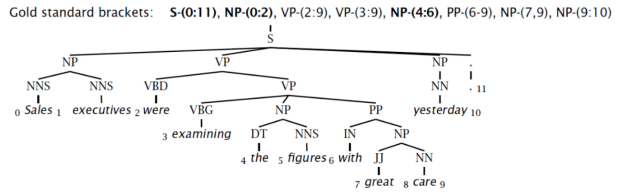
\includegraphics[width=0.95\textwidth]{assets/test2/gold_standard_brackets.png}
\end{figure}

\begin{figure}[!ht]
      \centering
      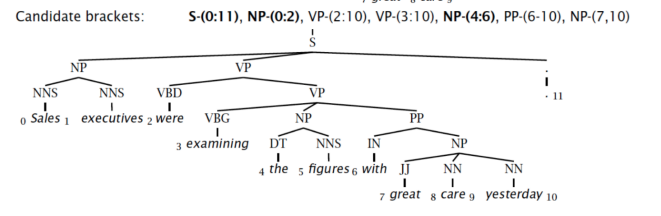
\includegraphics[width=0.95\textwidth]{assets/test2/candidate_brackets.png}
\end{figure}

% P8
\newpage
\section*{Question 8}
\textbf{[Points 5]} In transition-based parsing we see dependency structure were
provided, then why we need to parse the sentence while given the structures?

% P9
\newpage
\section*{Question 9}
\textbf{[Points 5]} What is CNF form? Why is Chomsky Normal Form used?

\begin{tabular}{lll}
      S & $\rightarrow$ & a X b X              \\
      X & $\rightarrow$ & a Y $|$ b Y $|$ null \\
      Y & $\rightarrow$ & X $|$ c              \\
\end{tabular}

Convert this CFG to CNF.

\textbf{Answer:}

\begin{figure}[!ht]
      \centering
      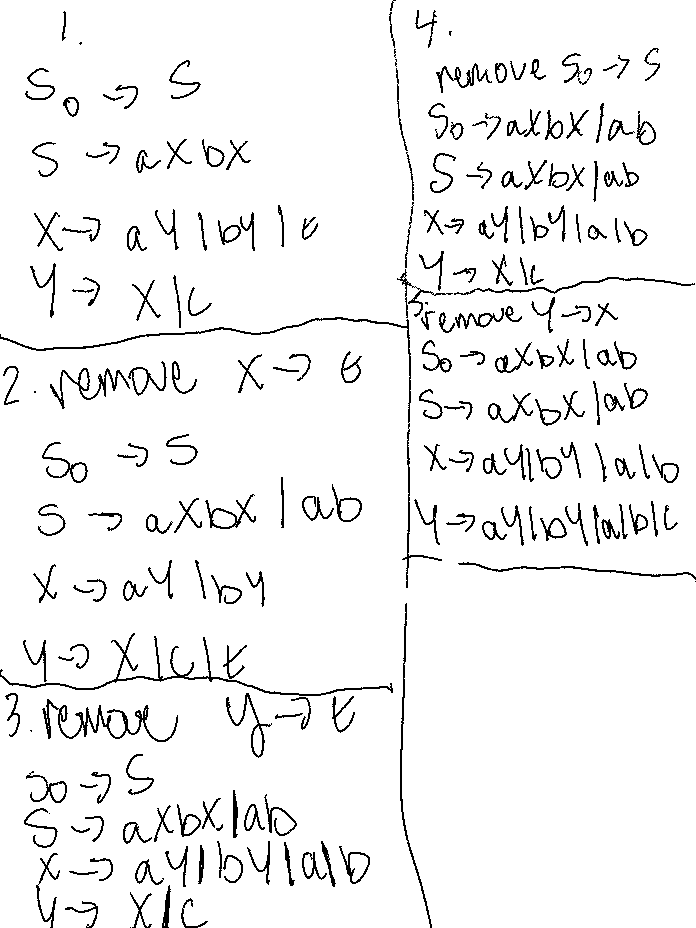
\includegraphics[width=0.6\textwidth]{assets/test2/p9a.png}
\end{figure}
\newpage

\begin{figure}[!ht]
      \centering
      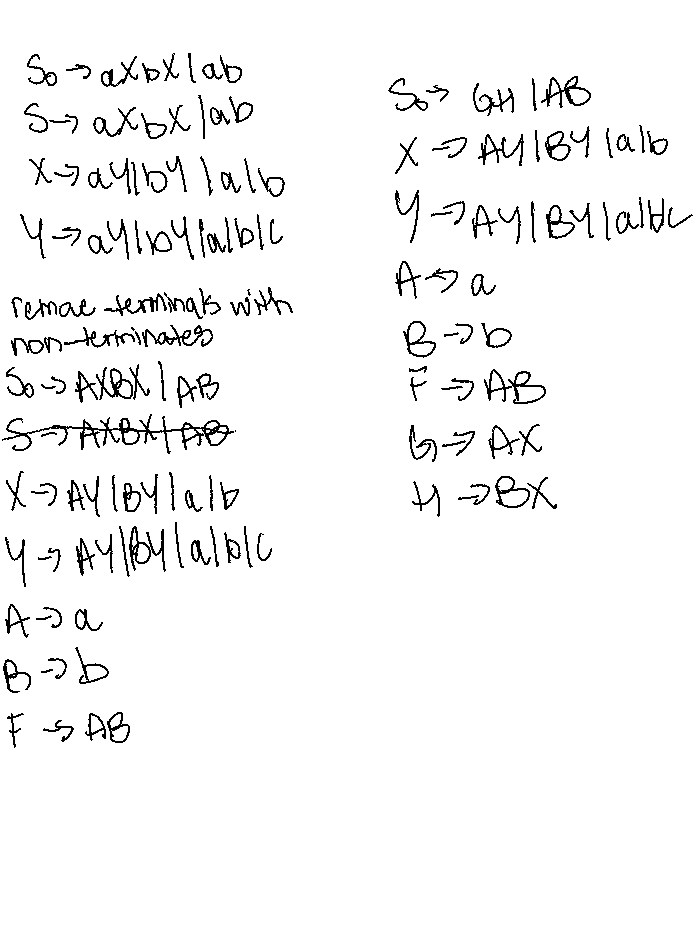
\includegraphics[width=0.6\textwidth]{assets/test2/p9b.png}
\end{figure}

% P10
\newpage
\section*{Question 10}
\textbf{[Points 5]} How would you encode sentence using deep neural network?
Show details architecture of your network with an example sentence.

\end{document}